\chapter{FPGA Implementation}
The General hardware design is explained using following the hierarchy graph.

\begin{figure}[H]
    \centering
    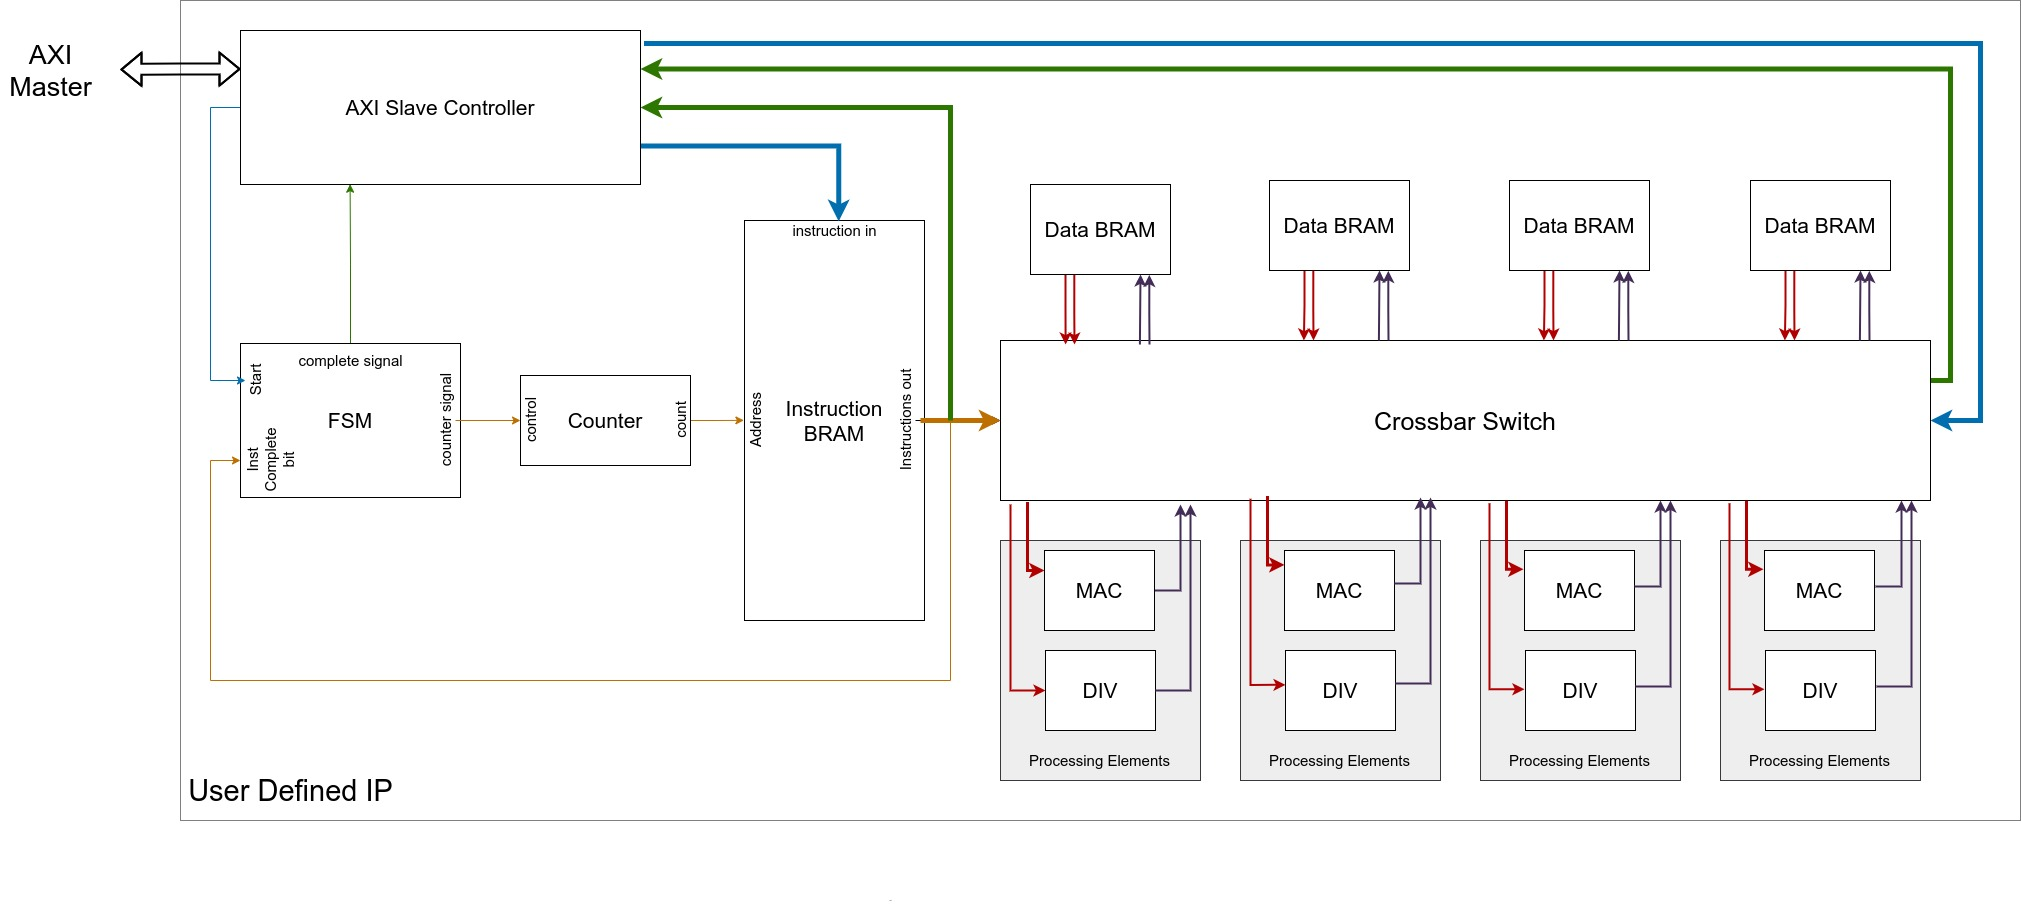
\includegraphics[width = \textwidth]{./FPGA_Implementation/OWN_Hardware.jpg}
    \caption{FPGA Implementation architecture}
    \label{fig:sym:flowGraph}
\end{figure}


The design uses Xilinx optimized IP, and a Crossbar switch box is used to interconnect the overall design as per the requirement for the accelerator. Following are the IPs used:-
\begin{itemize}
	\item Block Memory Generator (BRAM Unit) \cite{Xilinx_BRAM}
		\begin{itemize}
		\item Instruction BRAM (custom bit size)
		\item Data BRAM (float / double type)
		\end{itemize}
	\item Floating-point \cite{Xilinx_Floatpt}
		\begin{itemize}
			\item Fused Multiply-Add/Sub (MAC Unit)
			\item Division (DIV Unit)
		\end{itemize}
\end{itemize}

\section{Block Memory Generator (BRAM Unit) IP}

The Xilinx LogiCORE IP Block Memory Generator replaces the Dual Port Block Memory and Single Port Block Memory LogiCOREs but is not a direct drop-in replacement. It should be used in all new Xilinx designs. The core supports RAM and ROM functions over a wide range of widths and depths. Use this core to generate block memories with symmetric or asymmetric read and write port widths and centers that can perform simultaneous write operations to separate locations and simultaneous read operations from the exact location. For more information on differences in interface and feature support between this core and the Dual Port Block Memory and Single Port Block Memory LogiCOREs, please consult the datasheet.
\\
\\
The BRAM Units are used for instructions produced by the scheduler and storing $A$ and $LU$ Matrix values. The instructions BRAM used to select change the connection of crossbar switch in the design, which would lead to floating-point operations as per the schedule for Decomposition. The instructions BRAM is custom input/output bit as per the scheduler, and Data BRAM should be 32bit / 64bit as per the data type.

\section{Floating-point IP}
The Xilinx Floating-Point Operator is capable of being configured to provide a range of floating-point operations. The core offers addition, subtraction, accumulation, multiplication, fused multiply-add, division, reciprocal, square-root, reciprocal-square-root, absolute value, logarithm, exponential, compare, and conversion operations. High-speed, single-cycle throughput is provided at a wide range of word lengths, including half, single and double precision. DSP48 slices can be used with specific operations.
\\
\\
The floating-point IP is used to Multiply and Accumulate Unit and Divider Unit.
\\
\\
The LU factorization requires only a floating-point multiplier and subtract operation ($Result = C - AB$).The Xilinx's MAC units utilize on-chip DSP Slices to achieve higher performance.
\\
\\
The Xilinx Floating Point Divider IP utilizes some radix-2 SRT division algorithm variants and can not use DSP slices. These units are bulkier and therefore have to be deeply pipelined to operate. The speed grade of the target FPGA is one of the most dominating factors in determining the depth of the pipeline.


\section{Crossbar switch box}

The Crossbar switch box should connect any output port to an input port for  Data BRAMs, MAC, and DIV units. This can be achieved with a multiplexer. The select signals are provided by instructions BRAMs, which were produced by the scheduler. The number of multiplexers depends on Processing elements, the Number of Data BRAMs, and the number of ports at each BRAM.
\\
\\
The top-level design is developed into IP via AXI slave wrapper to connect soft-core and/or hard-core processors. The Crossbar switch box should instruct BRAM and Data BRAM to upload data/instruction and receive Matrix Decomposed Matrix.

\section{Shakti Board Integration (PARSHU)}
SHAKTI is an open-source initiative by the Reconfigurable Intelligent Systems Engineering (RISE) group at IIT-Madras. The SHAKTI initiative aims to build open-source production grade processors, complete System on Chips (SoCs), development boards, and a SHAKTI-based software platform. SHAKTI support on different development boards is crucial as this expands the hardware choice of FPGAs.The core has been completely developed using BSV (Bluespec System Verilog). As part of this effort, initially, two varieties of FPGA boards are being supported. They are Xilinx’s Arty7 35T and Arty7 100T.

In This Design, the targeted target is PARASHU\cite{Shakti_PARSHU} with the following specification.
\begin{itemize}
\item PARASHU is an SoC based on SHAKTI E-class \cite{Shakti_Eclass}
\item PARASHU is supported on Artix 7 100T board
\item It has an abridged version of the 32-bit E-class
\item Targeted frequency is 50 MHz
\item Storage 4 KB of ROM and 256 MB of DDR
\end{itemize}

This is the embedded class processor, built around a 3-stage in-order core. It is aimed at low-power and low compute applications and can run basic RTOSs like FreeRTOS and Zephyr (Chronos is also being ported and will be released soon). Typical market segments include: smart-cards, IoT sensors, motor controls, and robotic platforms.Based on the Following Map, it is configured.

\begin{table}[]
	\centering
	\begin{tabular}{|l|l|l|l|}
	\hline
	S.No. & Peripeheral   & Base Address Start & Base address End \\ \hline
	1     & Memory DDR    & 0x8000\_0000       & 0x8FFF\_FFFF     \\ \hline
	2     & Debug         & 0x0000\_0010       & 0x0000\_001F     \\ \hline
	3     & UART0         & 0x0001\_1300       & 0x0001\_1340     \\ \hline
	4     & UART1         & 0x0001\_1400       & 0x0001\_1440     \\ \hline
	5     & UART2         & 0x0001\_1500       & 0x0001\_1540     \\ \hline
	6     & I2C0          & 0x0004\_0000       & 0x0004\_00FF     \\ \hline
	7     & GPIO          & 0x0004\_0100       & 0x0004\_01FF     \\ \hline
	8     & CLINT         & 0x0200\_0000       & 0x020B\_FFFF     \\ \hline
	9     & PLIC          & 0x0C00\_0000       & 0x0C01\_001F     \\ \hline
	10    & PWM0          & 0x0030\_0000       & 0x0030\_00FF     \\ \hline
	11    & PWM1          & 0x0030\_0100       & 0x0030\_01FF     \\ \hline
	12    & PWM2          & 0x0030\_0200       & 0x0030\_02FF     \\ \hline
	13    & PWM3          & 0x0030\_0300       & 0x0030\_03FF     \\ \hline
	14    & PWM4          & 0x0030\_0400       & 0x0030\_04FF     \\ \hline
	15    & PWM5          & 0x0030\_0500       & 0x0030\_05FF     \\ \hline
	16    & SPI0          & 0x0002\_0000       & 0x0002\_00FF     \\ \hline
	17    & SPI1          & 0x0002\_0100       & 0x0002\_01FF     \\ \hline
	18    & I2C1          & 0x0004\_1400       & 0x0004\_14FF     \\ \hline
	19    & XADC          & 0x0004\_1000       & 0x0004\_13FF     \\ \hline
	20    & PinMux        & 0x0004\_1500       & 0x0004\_15FF     \\ \hline
	21    & Bot Rom       & 0x0000\_1000       & 0x0004\_15FF     \\ \hline
	22    & Custom Module & 0x0005\_0000       & 0x0005\_FFFF     \\ \hline
	\end{tabular}
%	\caption{Memory Map of Integrated Design}
\end{table}

The Integration of the accelerator is wrapped around AXI Slave protocol. Using the User manual\cite{Shakti_SDK} . The Basic structure of Shakti FPGA Project has the following directory structure:-

\begin{forest}
    for tree={
      font=\ttfamily,
      grow'=0,
      child anchor=west,
      parent anchor=south,
      anchor=west,
      calign=first,
      edge path={
        \noexpand\path [draw, \forestoption{edge}]
        (!u.south west) +(7.5pt,0) |- node[fill,inner sep=1.25pt] {} (.child anchor)\forestoption{edge label};
      },
      before typesetting nodes={
        if n=1
          {insert before={[,phantom]}}
          {}
      },
      fit=band,
      before computing xy={l=15pt},
    }
	[Shakti\_project\/
	[boot\-code : Boot related codes]
	[bsv\_build :  BSV related object files for Integration]
	[common\_bsv : Common BSV files for integration ]
	[common\_verilog : Verilog File generated using BSV]
	[devices : Devices that would be connected like BRAM\, PWM]
	[e-class : E-class core of the SHAKTI Processor family]
	[fabrics : interconnects based BSV files]
	[fpga\_project : Final Project and User-defined IPs]
	[tcl : Automated scripts for fpga\_project]
	[verilog : Final Build Verilog files and Cutsom Verilog Files]
	[Soc.bsv : Top Module Definition]
	[Soc.defines : Memory Maps of Design]
	[spi\_cluster and uart\_cluster : BSV files for SPI and UART Integration]]
\end{forest}

The alteration is done for the integration user-defined IP to the SHAKTI Processor by specifying the interconnecting cluster and protocol.



\begin{figure}
      \begin{subfigure}{.5\textwidth}
        \centering
        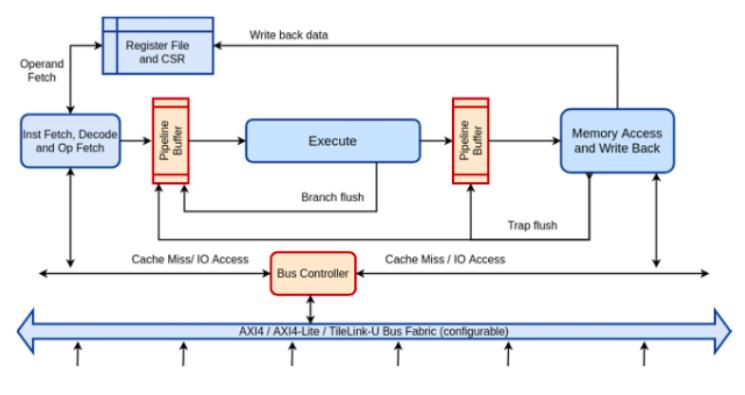
\includegraphics[width=.8\linewidth]{./FPGA_Implementation/Eclass.png}
        \caption{E Class Shakti Processor}
      %	\label{fig:sfig1}
        \end{subfigure}%
        \begin{subfigure}{.5\textwidth}
        \centering
        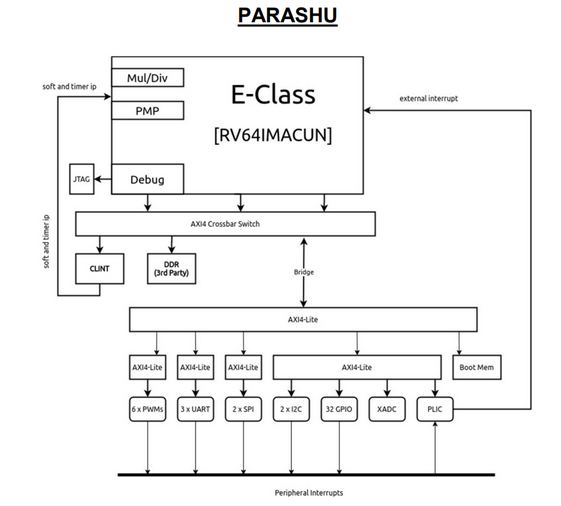
\includegraphics[width=.8\linewidth]{./FPGA_Implementation/parashu.png}
        \caption{Parashu Configuration of E Class Shakti Processor}
      %	\label{fig:sfig2}
        \end{subfigure}
        \caption{Shakti Processor E-Class based Parashu Configuration}
      %  \label{fig:fig}
\end{figure}

\section{Shakti SDK}

It is the open-source software development platform for SHAKTI. Clean separation between drivers, boot, core, and application layers.Driver support SPI, QSPI, PLIC, CLINT, UART, I2C, and PWM. Multiple sensors are connected and proven with SHAKTI-SDK. Standalone and Debug mode supported. Multilevel logging, Flash programming \& Dynamic memory management are supported. A single place for bare-metal application development, projects, and benchmarks.

\begin{figure}[H]
    \centering
    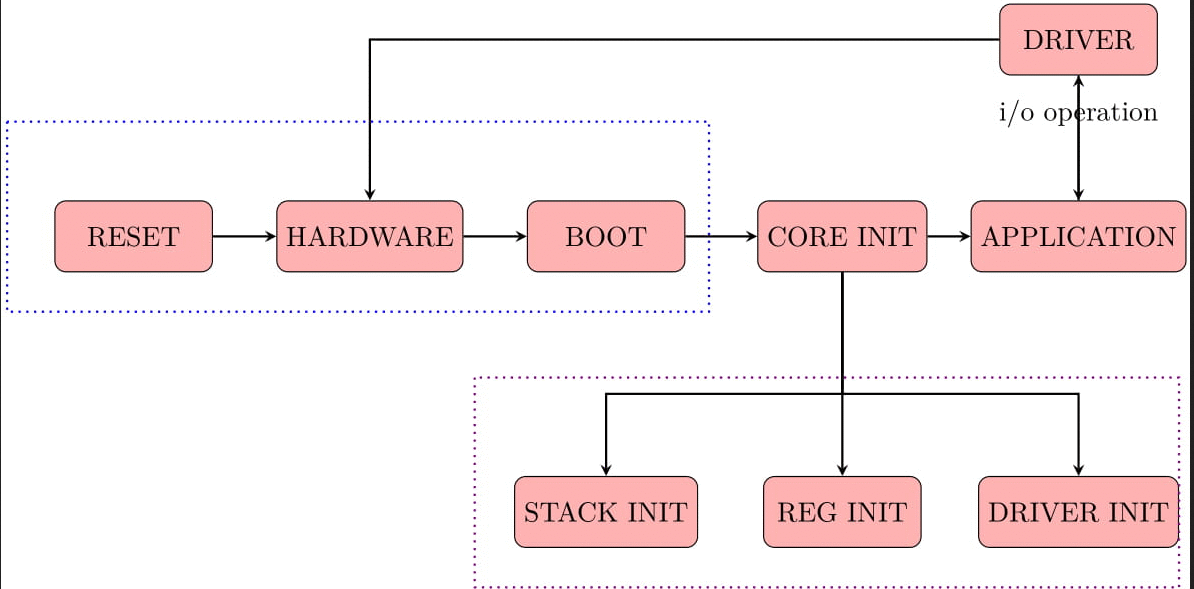
\includegraphics[width = 0.5\textwidth]{./FPGA_Implementation/SoftwareProgramflow.png}
    \caption{Software program flow}
    %\label{fig:sym:flowGraph}
\end{figure}

The SHAKTI-SDK is a C/C++ platform for developing applications over SHAKTI. The SDK has the necessary firmware code and framework to develop newer applications on the hardware. The framework is lightweight and customizable.

\begin{figure}[H]
    \centering
    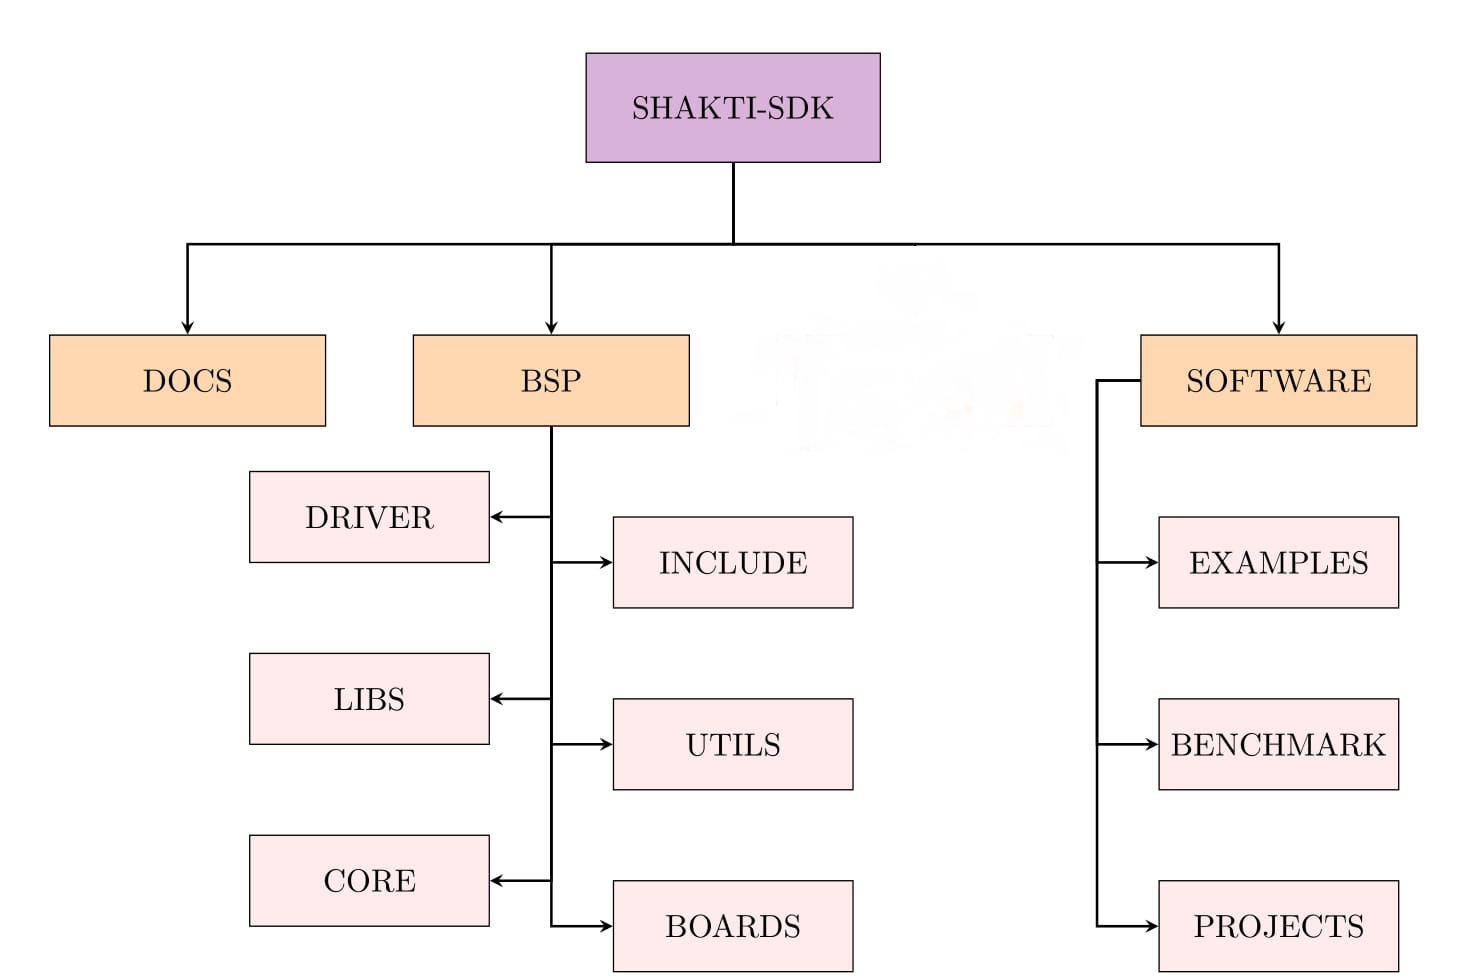
\includegraphics[width = 0.5\textwidth]{./FPGA_Implementation/SDK_architecture.jpg}
    \caption{SDK architecture}
    %\label{fig:sym:flowGraph}
\end{figure}

%Board Support Package
%\\
The BSP consists of system files and driver files for various devices. It contains specific platform-dependent definitions for each board. Essentially, the BSP is the layer above the hardware. It includes the following.

\begin{itemize}
	\itemsep0em 
	\item Drivers: The drivers are a set of software constructs that help software applications access the SoC devices. They are generally low-level APIs that execute a particular task in the hardware.
	\item Include: The board independtn varabole/macro definitios adn declarations.
	\item Libs: The library utilities and the boot code.
	\item Core: The core usually has functions related to the startup codes, trap handlers and interrupt vectors. The code is related to memory initialization.
	\item Utils: This contains the code related to standalone mode features of the Software 
\end{itemize}

%Software and Shaki tools
%\\
The software directory provides a platform for developing various applications independent of the underlying BSP. All the applications/projects developed in SHAKTI-SDK reside in this directory. SHAKTI uses the RISC-V toolchain. A software toolchain to create assembly instructions \& sequences for execution in both a simulator and target FPGA. The Shakti Integration was check on varities of becnhmark as shown in Table of Performance variation with the number of Ports in BRAMs.

\begin{table}[h]
	\centering
	\begin{tabular}{|lllll|}
	\hline
	\multicolumn{1}{|l|}{Matrix Name} & \multicolumn{1}{l|}{Kind of Problem} & \multicolumn{1}{l|}{NNZ} & \multicolumn{1}{l|}{16 Single-Port} & 8 Dual-Port \\ \hline
	Trefethen\_20b & Combinatorial               & 147  & 375  & 336  \\
	rajat11        & Circuit Simulation          & 665  & 463  & 442  \\
	bwm200         & Chemical Process & 796  & 4002 & 3995 \\
	494\_bus       & Power Network               & 1666 & 1157 & 1044 \\
	mhdb416        & Electromagnetics            & 2312 & 2007 & 1821 \\ \hline
	\end{tabular}
	\caption{Performance variation with the number of Ports in BRAMs}
\end{table}
%\pagebreak